% !TeX root = ../thuthesis-example.tex

\chapter{SUMMARY, DISCUSSION AND FUTURE DIRECTIONS}

\section{Discussion and future directions}

The work's novelty lies in the fact that there are no studies on the creation and interaction of devices for a VR-IoT environment. All similar researches concentrate on controlling IoT devices using Virtual reality headsets.
The author hopes to continue working on the platform in the future in the university laboratory. The possible timeline for the development has been created.

\begin{figure}
  \centering
  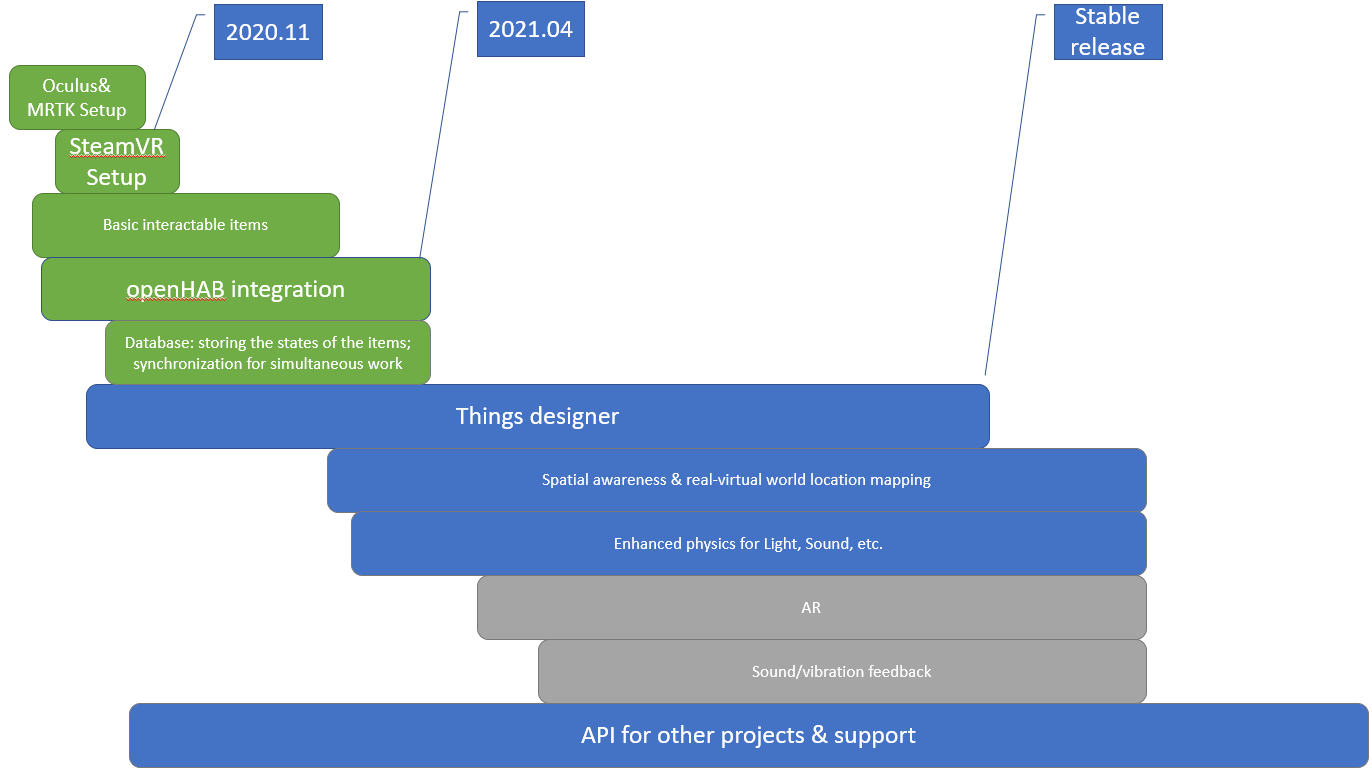
\includegraphics[width=0.9\linewidth]{figures/Timeline.png}
  \caption{Timeline}
  \label{fig:Timeline-figure}
\end{figure}

As seen in (Figure~\ref{fig:Timeline-figure}), the development started from providing support for Virtual reality headsets. The next step was implementing openHAB and database support to perform simultaneous interaction in the same environment by several App instances. In the text of this research, it was discussed that these two tasks could be considered complete. However, the Things designer is not fully developed since further research is needed to provide a wider variety of supported Widgets and Items.

Mixed Reality toolkit can provide real-world environmental awareness for apps running on Hololens. It is already possible to run NUIX-Studio APP on Hololens, although it has not yet been tested. Using spatial awareness, NUIX-Studio App will be possible to align virtual Widgets onto IoT devices. Developing real-virtual world location mapping for the Widgets for Virtual reality will be required as well.

Currently, only advanced illumination can be computed on the NUIX-Studio APP. Researchers may need more accurate data to create new IoT devices. In this case, Unity Game Engine can be extended with more precise light, sound, and other physics support.

Providing AR support requires adding new interaction techniques and training Deep learning models to provide object recognition. Users can use both AR and VR to research new IoT devices, with AR being responsible for retrieving the coordinates of the devices from the real world (by OpenCV, Tensoflow Graphics, etc.), and VR for visualizing environments that are difficult or impossible to implement in AR (for example, flying on a plane or driving a car).

Augmented reality, Virtual reality, and Mixed Reality are not the only interfaces to interact with IoT in the virtual world. What if the feedback from IoT devices only by sound and vibrations is provided? NUIX-Studio can be adapted for such limitations. One of the example usages of this approach is research for visually impaired people in an IoT environment.

During the entire development cycle, an API must be developed for embedding external developments into the platform, including projects of HCI Lab students. 

\section{Summary}

The purpose of the work is completed: a platform for creating new devices for the existing IoT world in Virtual reality is presented, which helps develop new devices. It has been shown that it allows this to be done both theoretically and practically.